% Options for packages loaded elsewhere
\PassOptionsToPackage{unicode}{hyperref}
\PassOptionsToPackage{hyphens}{url}
%
\documentclass[
]{article}
\usepackage{amsmath,amssymb}
\usepackage{iftex}
\ifPDFTeX
  \usepackage[T1]{fontenc}
  \usepackage[utf8]{inputenc}
  \usepackage{textcomp} % provide euro and other symbols
\else % if luatex or xetex
  \usepackage{unicode-math} % this also loads fontspec
  \defaultfontfeatures{Scale=MatchLowercase}
  \defaultfontfeatures[\rmfamily]{Ligatures=TeX,Scale=1}
\fi
\usepackage{lmodern}
\ifPDFTeX\else
  % xetex/luatex font selection
\fi
% Use upquote if available, for straight quotes in verbatim environments
\IfFileExists{upquote.sty}{\usepackage{upquote}}{}
\IfFileExists{microtype.sty}{% use microtype if available
  \usepackage[]{microtype}
  \UseMicrotypeSet[protrusion]{basicmath} % disable protrusion for tt fonts
}{}
\makeatletter
\@ifundefined{KOMAClassName}{% if non-KOMA class
  \IfFileExists{parskip.sty}{%
    \usepackage{parskip}
  }{% else
    \setlength{\parindent}{0pt}
    \setlength{\parskip}{6pt plus 2pt minus 1pt}}
}{% if KOMA class
  \KOMAoptions{parskip=half}}
\makeatother
\usepackage{xcolor}
\usepackage[margin=1in]{geometry}
\usepackage{color}
\usepackage{fancyvrb}
\newcommand{\VerbBar}{|}
\newcommand{\VERB}{\Verb[commandchars=\\\{\}]}
\DefineVerbatimEnvironment{Highlighting}{Verbatim}{commandchars=\\\{\}}
% Add ',fontsize=\small' for more characters per line
\usepackage{framed}
\definecolor{shadecolor}{RGB}{248,248,248}
\newenvironment{Shaded}{\begin{snugshade}}{\end{snugshade}}
\newcommand{\AlertTok}[1]{\textcolor[rgb]{0.94,0.16,0.16}{#1}}
\newcommand{\AnnotationTok}[1]{\textcolor[rgb]{0.56,0.35,0.01}{\textbf{\textit{#1}}}}
\newcommand{\AttributeTok}[1]{\textcolor[rgb]{0.13,0.29,0.53}{#1}}
\newcommand{\BaseNTok}[1]{\textcolor[rgb]{0.00,0.00,0.81}{#1}}
\newcommand{\BuiltInTok}[1]{#1}
\newcommand{\CharTok}[1]{\textcolor[rgb]{0.31,0.60,0.02}{#1}}
\newcommand{\CommentTok}[1]{\textcolor[rgb]{0.56,0.35,0.01}{\textit{#1}}}
\newcommand{\CommentVarTok}[1]{\textcolor[rgb]{0.56,0.35,0.01}{\textbf{\textit{#1}}}}
\newcommand{\ConstantTok}[1]{\textcolor[rgb]{0.56,0.35,0.01}{#1}}
\newcommand{\ControlFlowTok}[1]{\textcolor[rgb]{0.13,0.29,0.53}{\textbf{#1}}}
\newcommand{\DataTypeTok}[1]{\textcolor[rgb]{0.13,0.29,0.53}{#1}}
\newcommand{\DecValTok}[1]{\textcolor[rgb]{0.00,0.00,0.81}{#1}}
\newcommand{\DocumentationTok}[1]{\textcolor[rgb]{0.56,0.35,0.01}{\textbf{\textit{#1}}}}
\newcommand{\ErrorTok}[1]{\textcolor[rgb]{0.64,0.00,0.00}{\textbf{#1}}}
\newcommand{\ExtensionTok}[1]{#1}
\newcommand{\FloatTok}[1]{\textcolor[rgb]{0.00,0.00,0.81}{#1}}
\newcommand{\FunctionTok}[1]{\textcolor[rgb]{0.13,0.29,0.53}{\textbf{#1}}}
\newcommand{\ImportTok}[1]{#1}
\newcommand{\InformationTok}[1]{\textcolor[rgb]{0.56,0.35,0.01}{\textbf{\textit{#1}}}}
\newcommand{\KeywordTok}[1]{\textcolor[rgb]{0.13,0.29,0.53}{\textbf{#1}}}
\newcommand{\NormalTok}[1]{#1}
\newcommand{\OperatorTok}[1]{\textcolor[rgb]{0.81,0.36,0.00}{\textbf{#1}}}
\newcommand{\OtherTok}[1]{\textcolor[rgb]{0.56,0.35,0.01}{#1}}
\newcommand{\PreprocessorTok}[1]{\textcolor[rgb]{0.56,0.35,0.01}{\textit{#1}}}
\newcommand{\RegionMarkerTok}[1]{#1}
\newcommand{\SpecialCharTok}[1]{\textcolor[rgb]{0.81,0.36,0.00}{\textbf{#1}}}
\newcommand{\SpecialStringTok}[1]{\textcolor[rgb]{0.31,0.60,0.02}{#1}}
\newcommand{\StringTok}[1]{\textcolor[rgb]{0.31,0.60,0.02}{#1}}
\newcommand{\VariableTok}[1]{\textcolor[rgb]{0.00,0.00,0.00}{#1}}
\newcommand{\VerbatimStringTok}[1]{\textcolor[rgb]{0.31,0.60,0.02}{#1}}
\newcommand{\WarningTok}[1]{\textcolor[rgb]{0.56,0.35,0.01}{\textbf{\textit{#1}}}}
\usepackage{graphicx}
\makeatletter
\def\maxwidth{\ifdim\Gin@nat@width>\linewidth\linewidth\else\Gin@nat@width\fi}
\def\maxheight{\ifdim\Gin@nat@height>\textheight\textheight\else\Gin@nat@height\fi}
\makeatother
% Scale images if necessary, so that they will not overflow the page
% margins by default, and it is still possible to overwrite the defaults
% using explicit options in \includegraphics[width, height, ...]{}
\setkeys{Gin}{width=\maxwidth,height=\maxheight,keepaspectratio}
% Set default figure placement to htbp
\makeatletter
\def\fps@figure{htbp}
\makeatother
\setlength{\emergencystretch}{3em} % prevent overfull lines
\providecommand{\tightlist}{%
  \setlength{\itemsep}{0pt}\setlength{\parskip}{0pt}}
\setcounter{secnumdepth}{-\maxdimen} % remove section numbering
\ifLuaTeX
  \usepackage{selnolig}  % disable illegal ligatures
\fi
\IfFileExists{bookmark.sty}{\usepackage{bookmark}}{\usepackage{hyperref}}
\IfFileExists{xurl.sty}{\usepackage{xurl}}{} % add URL line breaks if available
\urlstyle{same}
\hypersetup{
  pdftitle={Meta-Analysis for Longevity Summary Excluding HUM251},
  pdfauthor={Fay Frost},
  hidelinks,
  pdfcreator={LaTeX via pandoc}}

\title{Meta-Analysis for Longevity Summary Excluding HUM251}
\author{Fay Frost}
\date{}

\begin{document}
\maketitle

\hypertarget{summary}{%
\section{1. Summary}\label{summary}}

This document reports the process taken in the model fitting stage of
the meta-analysis in thermal longevity.

\hypertarget{setup}{%
\section{2. Setup}\label{setup}}

We first read in our data and select all of the effect sizes related to
longevity. We do this using the following code.

\begin{Shaded}
\begin{Highlighting}[]
\DocumentationTok{\#\#\# Read in effect size data}
\NormalTok{effectdata }\OtherTok{\textless{}{-}} \FunctionTok{read.csv}\NormalTok{(}\StringTok{"Survival project all pairwise.es.csv"}\NormalTok{)}
\NormalTok{longdata\_warm }\OtherTok{\textless{}{-}} \FunctionTok{subset}\NormalTok{(effectdata, Trait.category }\SpecialCharTok{==} \StringTok{"Longevity"} \SpecialCharTok{\&}
\NormalTok{    warm.cool }\SpecialCharTok{==} \StringTok{"Warm"}\NormalTok{)}
\NormalTok{longdata\_cool }\OtherTok{\textless{}{-}} \FunctionTok{subset}\NormalTok{(effectdata, Trait.category }\SpecialCharTok{==} \StringTok{"Longevity"} \SpecialCharTok{\&}
\NormalTok{    warm.cool }\SpecialCharTok{==} \StringTok{"Cool"}\NormalTok{)}

\NormalTok{alllong }\OtherTok{\textless{}{-}} \FunctionTok{rbind}\NormalTok{(longdata\_warm, longdata\_cool)}

\DocumentationTok{\#\#\# select data for analysis}
\NormalTok{rdata }\OtherTok{\textless{}{-}}\NormalTok{ alllong}

\NormalTok{rdata }\OtherTok{\textless{}{-}} \FunctionTok{subset}\NormalTok{(rdata, Paper.code }\SpecialCharTok{!=} \StringTok{"HUM251"}\NormalTok{)}

\NormalTok{rdata }\OtherTok{\textless{}{-}}\NormalTok{ rdata }\SpecialCharTok{\%\textgreater{}\%}
    \FunctionTok{mutate}\NormalTok{(}\AttributeTok{c\_treattemp =}\NormalTok{ treattemp }\SpecialCharTok{{-}} \DecValTok{25}\NormalTok{)}
\end{Highlighting}
\end{Shaded}

Next we create new columns in our dataframe which will serve as random
factors in our multi-level meta analysis models. The following
initialises four new columns, namely ``obs'', ``study\_code'',
``Species.phylo'' and ``species''. Lastly, we create a column name
``precision'' which is equal to the inverse standard error.

\begin{Shaded}
\begin{Highlighting}[]
\DocumentationTok{\#\#\# Create random factors into data frame}
\NormalTok{rdata}\SpecialCharTok{$}\NormalTok{obs }\OtherTok{\textless{}{-}} \FunctionTok{factor}\NormalTok{(}\FunctionTok{c}\NormalTok{(}\DecValTok{1}\SpecialCharTok{:}\FunctionTok{nrow}\NormalTok{(rdata)))  }\CommentTok{\# Unique observation code}
\NormalTok{rdata}\SpecialCharTok{$}\NormalTok{study\_code }\OtherTok{\textless{}{-}} \FunctionTok{factor}\NormalTok{(rdata}\SpecialCharTok{$}\NormalTok{Paper.code)  }\CommentTok{\# Model requires column names study\_code }
\NormalTok{rdata}\SpecialCharTok{$}\NormalTok{Species.phylo }\OtherTok{\textless{}{-}} \FunctionTok{factor}\NormalTok{(rdata}\SpecialCharTok{$}\NormalTok{Species.latin)  }\CommentTok{\# Species names for phylo matrix}
\NormalTok{rdata}\SpecialCharTok{$}\NormalTok{species }\OtherTok{\textless{}{-}} \FunctionTok{factor}\NormalTok{(rdata}\SpecialCharTok{$}\NormalTok{Species.latin)  }\CommentTok{\# Another species column for random factor }

\NormalTok{precision }\OtherTok{\textless{}{-}} \FunctionTok{sqrt}\NormalTok{(}\DecValTok{1}\SpecialCharTok{/}\NormalTok{rdata}\SpecialCharTok{$}\NormalTok{v)  }\CommentTok{\# inverse standard error }
\NormalTok{rdata[, }\StringTok{"precision"}\NormalTok{] }\OtherTok{\textless{}{-}}\NormalTok{ precision}
\end{Highlighting}
\end{Shaded}

The number of species and total number of studies present in the data
are as follows.

\begin{Shaded}
\begin{Highlighting}[]
\FunctionTok{nlevels}\NormalTok{(rdata}\SpecialCharTok{$}\NormalTok{species)  }\CommentTok{\# Check number of species}
\end{Highlighting}
\end{Shaded}

\begin{verbatim}
## [1] 289
\end{verbatim}

\begin{Shaded}
\begin{Highlighting}[]
\FunctionTok{nlevels}\NormalTok{(rdata}\SpecialCharTok{$}\NormalTok{study\_code)  }\CommentTok{\# Check number of studies}
\end{Highlighting}
\end{Shaded}

\begin{verbatim}
## [1] 315
\end{verbatim}

\newpage

The final stage in the setup is to import a phylogentic tree of the
data. Below is the code used to produce the tree and a plot of the tree
itself.

\begin{Shaded}
\begin{Highlighting}[]
\DocumentationTok{\#\# import tree from map}
\NormalTok{tree1 }\OtherTok{\textless{}{-}} \FunctionTok{read.nexus}\NormalTok{(}\StringTok{"all\_longevity\_excHUM251\_tree.nex"}\NormalTok{)}
\NormalTok{tree\_grafen }\OtherTok{=} \FunctionTok{compute.brlen}\NormalTok{(tree1, }\AttributeTok{method =} \StringTok{"Grafen"}\NormalTok{, }\AttributeTok{power =} \DecValTok{1}\NormalTok{)}
\NormalTok{phylo\_matrix }\OtherTok{\textless{}{-}} \FunctionTok{vcv}\NormalTok{(tree\_grafen, }\AttributeTok{cor =} \ConstantTok{TRUE}\NormalTok{, }\AttributeTok{model =} \StringTok{"Brownian"}\NormalTok{)  }\CommentTok{\# Make phylogenetic matrix}
\end{Highlighting}
\end{Shaded}

\begin{verbatim}
## character(0)
\end{verbatim}

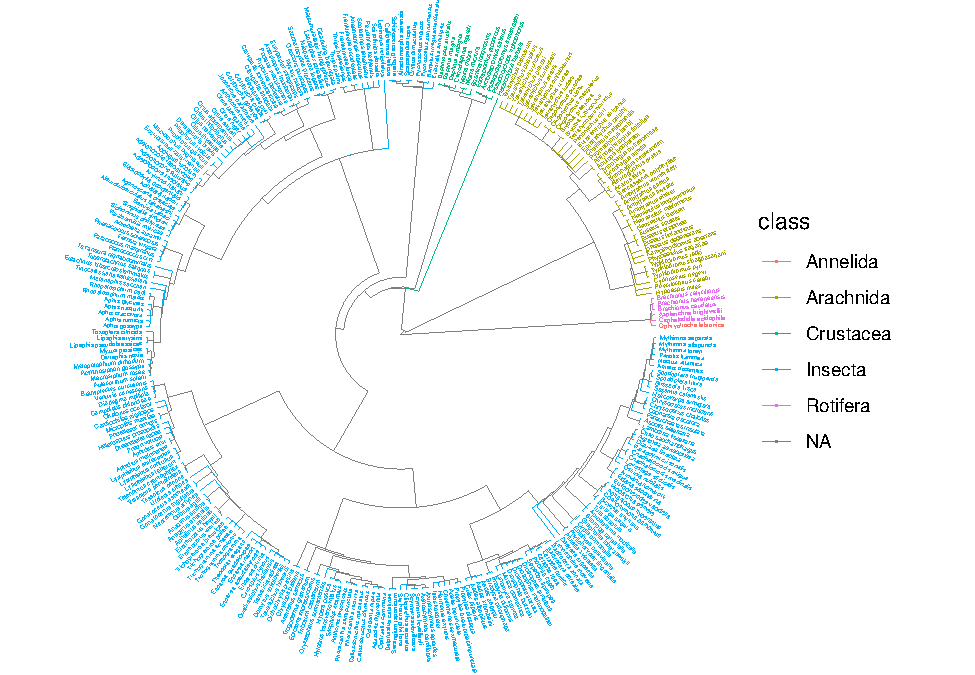
\includegraphics{meta_analysis_longevity_files/figure-latex/unnamed-chunk-6-1.pdf}

\newpage

\hypertarget{random-effects-models}{%
\section{3. Random effects models}\label{random-effects-models}}

In this section we determine which random effects to include in our
model. For each model I have provided the code used to specify the
structure of the model and a summary of the results. We begin with a
model that includes all of the random factors we created earlier.

\begin{Shaded}
\begin{Highlighting}[]
\CommentTok{\# Adding four random factors}
\NormalTok{meta2 }\OtherTok{\textless{}{-}} \FunctionTok{rma.mv}\NormalTok{(es, v, }\AttributeTok{random =} \FunctionTok{list}\NormalTok{(}\SpecialCharTok{\textasciitilde{}}\DecValTok{1} \SpecialCharTok{|}\NormalTok{ Species.phylo, }\SpecialCharTok{\textasciitilde{}}\DecValTok{1} \SpecialCharTok{|}
\NormalTok{    species, }\SpecialCharTok{\textasciitilde{}}\DecValTok{1} \SpecialCharTok{|}\NormalTok{ study\_code, }\SpecialCharTok{\textasciitilde{}}\DecValTok{1} \SpecialCharTok{|}\NormalTok{ obs), }\AttributeTok{R =} \FunctionTok{list}\NormalTok{(}\AttributeTok{Species.phylo =}\NormalTok{ phylo\_matrix),}
    \AttributeTok{test =} \StringTok{"t"}\NormalTok{, }\AttributeTok{dfs =} \StringTok{"contain"}\NormalTok{, }\AttributeTok{data =}\NormalTok{ rdata, }\AttributeTok{method =} \StringTok{"REML"}\NormalTok{)}
\end{Highlighting}
\end{Shaded}

\begin{Shaded}
\begin{Highlighting}[]
\FunctionTok{summary}\NormalTok{(meta2)}
\end{Highlighting}
\end{Shaded}

\begin{verbatim}
## 
## Multivariate Meta-Analysis Model (k = 1377; method: REML)
## 
##     logLik    Deviance         AIC         BIC        AICc   
## -3561.6881   7123.3763   7133.3763   7159.5110   7133.4201   
## 
## Variance Components:
## 
##             estim    sqrt  nlvls  fixed         factor    R 
## sigma^2.1  0.0000  0.0000    289     no  Species.phylo  yes 
## sigma^2.2  0.0000  0.0003    289     no        species   no 
## sigma^2.3  0.9600  0.9798    315     no     study_code   no 
## sigma^2.4  7.6881  2.7727   1377     no            obs   no 
## 
## Test for Heterogeneity:
## Q(df = 1376) = 51290.4596, p-val < .0001
## 
## Model Results:
## 
## estimate      se     zval    pval    ci.lb   ci.ub    
##  -0.1761  0.0983  -1.7919  0.0732  -0.3687  0.0165  . 
## 
## ---
## Signif. codes:  0 '***' 0.001 '**' 0.01 '*' 0.05 '.' 0.1 ' ' 1
\end{verbatim}

\begin{Shaded}
\begin{Highlighting}[]
\FunctionTok{i2\_ml}\NormalTok{(meta2, }\AttributeTok{method =} \FunctionTok{c}\NormalTok{(}\StringTok{"ratio"}\NormalTok{))  }\CommentTok{\# Heterogeneity at each random factor level}
\end{Highlighting}
\end{Shaded}

\begin{verbatim}
##         I2_Total I2_Species.phylo       I2_species    I2_study_code           I2_obs 
##     9.908349e+01     2.668394e-08     8.399927e-07     1.099874e+01     8.808476e+01
\end{verbatim}

\hypertarget{accounting-for-non-independence-of-data-points-from-the-same-experiment}{%
\subsection{Accounting for non-independence of data points from the same
experiment}\label{accounting-for-non-independence-of-data-points-from-the-same-experiment}}

The data has a nested structure. Each study (study\_code) may have a
number of experiments (effect.size.code) which share a common control
temperature. Each effect size has its own unique code, obs. Effect sizes
from the same experiment which share a control temperature are thought
to be non-independent. The following code create a covariance matrix
``VCV\_shared'' which assumes a correlation of 0.5 between effect sizes
from the same experiment. We include this structure in our proceeding
models.

\begin{Shaded}
\begin{Highlighting}[]
\NormalTok{rdata}\SpecialCharTok{$}\NormalTok{shared\_control }\OtherTok{\textless{}{-}} \FunctionTok{factor}\NormalTok{(rdata}\SpecialCharTok{$}\NormalTok{Effect.size.code)}
\NormalTok{vcv\_shared }\OtherTok{\textless{}{-}} \FunctionTok{impute\_covariance\_matrix}\NormalTok{(}\AttributeTok{vi =}\NormalTok{ rdata}\SpecialCharTok{$}\NormalTok{v, }\AttributeTok{cluster =}\NormalTok{ rdata}\SpecialCharTok{$}\NormalTok{shared\_control,}
    \AttributeTok{r =} \FloatTok{0.5}\NormalTok{)}
\end{Highlighting}
\end{Shaded}

\begin{Shaded}
\begin{Highlighting}[]
\CommentTok{\# Add new variance matrix into the mixed{-}effects}
\CommentTok{\# meta{-}analysis model}
\NormalTok{meta3 }\OtherTok{\textless{}{-}} \FunctionTok{rma.mv}\NormalTok{(es, vcv\_shared, }\AttributeTok{random =} \FunctionTok{list}\NormalTok{(}\SpecialCharTok{\textasciitilde{}}\DecValTok{1} \SpecialCharTok{|}\NormalTok{ Species.phylo,}
    \SpecialCharTok{\textasciitilde{}}\DecValTok{1} \SpecialCharTok{|}\NormalTok{ species, }\SpecialCharTok{\textasciitilde{}}\DecValTok{1} \SpecialCharTok{|}\NormalTok{ study\_code, }\SpecialCharTok{\textasciitilde{}}\DecValTok{1} \SpecialCharTok{|}\NormalTok{ obs), }\AttributeTok{test =} \StringTok{"t"}\NormalTok{, }\AttributeTok{dfs =} \StringTok{"contain"}\NormalTok{,}
    \AttributeTok{R =} \FunctionTok{list}\NormalTok{(}\AttributeTok{Species.phylo =}\NormalTok{ phylo\_matrix), }\AttributeTok{data =}\NormalTok{ rdata, }\AttributeTok{method =} \StringTok{"REML"}\NormalTok{)}
\end{Highlighting}
\end{Shaded}

\begin{Shaded}
\begin{Highlighting}[]
\FunctionTok{summary}\NormalTok{(meta3)}
\end{Highlighting}
\end{Shaded}

\begin{verbatim}
## 
## Multivariate Meta-Analysis Model (k = 1377; method: REML)
## 
##     logLik    Deviance         AIC         BIC        AICc   
## -3550.7026   7101.4053   7111.4053   7137.5399   7111.4491   
## 
## Variance Components:
## 
##             estim    sqrt  nlvls  fixed         factor    R 
## sigma^2.1  0.0000  0.0000    289     no  Species.phylo  yes 
## sigma^2.2  0.0000  0.0003    289     no        species   no 
## sigma^2.3  0.6854  0.8279    315     no     study_code   no 
## sigma^2.4  7.9521  2.8200   1377     no            obs   no 
## 
## Test for Heterogeneity:
## Q(df = 1376) = 69509.3558, p-val < .0001
## 
## Model Results:
## 
## estimate      se     zval    pval    ci.lb    ci.ub    
##  -0.1880  0.0950  -1.9800  0.0477  -0.3742  -0.0019  * 
## 
## ---
## Signif. codes:  0 '***' 0.001 '**' 0.01 '*' 0.05 '.' 0.1 ' ' 1
\end{verbatim}

\begin{Shaded}
\begin{Highlighting}[]
\FunctionTok{i2\_ml}\NormalTok{(meta3, }\AttributeTok{method =} \FunctionTok{c}\NormalTok{(}\StringTok{"ratio"}\NormalTok{))  }\CommentTok{\# Heterogeneity at each random factor level}
\end{Highlighting}
\end{Shaded}

\begin{verbatim}
##         I2_Total I2_Species.phylo       I2_species    I2_study_code           I2_obs 
##     9.908239e+01     6.530186e-11     7.656392e-07     7.862756e+00     9.121964e+01
\end{verbatim}

\newpage

\hypertarget{model-without-phylogeny}{%
\subsection{Model without phylogeny}\label{model-without-phylogeny}}

The variance-covariance matrix for phylogenetic relatedness of included
species has now been excluded as a random effect in the model
(Chamberlain et al., 2012) as its inclusion did not improve model fit
and the phylogenetic signal was very weak.

\begin{Shaded}
\begin{Highlighting}[]
\DocumentationTok{\#\# without phylogeny}
\NormalTok{meta5 }\OtherTok{\textless{}{-}} \FunctionTok{rma.mv}\NormalTok{(es, VCV\_shared, }\AttributeTok{random =} \FunctionTok{list}\NormalTok{(}\SpecialCharTok{\textasciitilde{}}\DecValTok{1} \SpecialCharTok{|}\NormalTok{ species, }\SpecialCharTok{\textasciitilde{}}\DecValTok{1} \SpecialCharTok{|}
\NormalTok{    study\_code, }\SpecialCharTok{\textasciitilde{}}\DecValTok{1} \SpecialCharTok{|}\NormalTok{ obs), }\AttributeTok{test =} \StringTok{"t"}\NormalTok{, }\AttributeTok{dfs =} \StringTok{"contain"}\NormalTok{, }\AttributeTok{data =}\NormalTok{ rdata,}
    \AttributeTok{method =} \StringTok{"REML"}\NormalTok{)}
\end{Highlighting}
\end{Shaded}

\begin{Shaded}
\begin{Highlighting}[]
\FunctionTok{summary}\NormalTok{(meta5)}
\end{Highlighting}
\end{Shaded}

\begin{verbatim}
## 
## Multivariate Meta-Analysis Model (k = 1377; method: REML)
## 
##     logLik    Deviance         AIC         BIC        AICc   
## -3550.7026   7101.4053   7109.4053   7130.3130   7109.4344   
## 
## Variance Components:
## 
##             estim    sqrt  nlvls  fixed      factor 
## sigma^2.1  0.0000  0.0003    289     no     species 
## sigma^2.2  0.6854  0.8279    315     no  study_code 
## sigma^2.3  7.9521  2.8200   1377     no         obs 
## 
## Test for Heterogeneity:
## Q(df = 1376) = 69509.3558, p-val < .0001
## 
## Model Results:
## 
## estimate      se     zval    pval    ci.lb    ci.ub    
##  -0.1880  0.0950  -1.9800  0.0477  -0.3742  -0.0019  * 
## 
## ---
## Signif. codes:  0 '***' 0.001 '**' 0.01 '*' 0.05 '.' 0.1 ' ' 1
\end{verbatim}

\begin{Shaded}
\begin{Highlighting}[]
\FunctionTok{i2\_ml}\NormalTok{(meta5, }\AttributeTok{method =} \FunctionTok{c}\NormalTok{(}\StringTok{"ratio"}\NormalTok{))  }\CommentTok{\# Heterogeneity at each random factor level}
\end{Highlighting}
\end{Shaded}

\begin{verbatim}
##      I2_Total    I2_species I2_study_code        I2_obs 
##  9.908239e+01  9.360291e-07  7.862751e+00  9.121964e+01
\end{verbatim}

\newpage

\hypertarget{model-without-phylogeny-or-species}{%
\subsection{Model without phylogeny or
species}\label{model-without-phylogeny-or-species}}

\begin{Shaded}
\begin{Highlighting}[]
\DocumentationTok{\#\# without phylogeny or species}
\NormalTok{meta4 }\OtherTok{\textless{}{-}} \FunctionTok{rma.mv}\NormalTok{(es, VCV\_shared, }\AttributeTok{random =} \FunctionTok{list}\NormalTok{(}\SpecialCharTok{\textasciitilde{}}\DecValTok{1} \SpecialCharTok{|}\NormalTok{ study\_code,}
    \SpecialCharTok{\textasciitilde{}}\DecValTok{1} \SpecialCharTok{|}\NormalTok{ obs), }\AttributeTok{data =}\NormalTok{ rdata, }\AttributeTok{test =} \StringTok{"t"}\NormalTok{, }\AttributeTok{dfs =} \StringTok{"contain"}\NormalTok{, }\AttributeTok{method =} \StringTok{"REML"}\NormalTok{)}
\end{Highlighting}
\end{Shaded}

\begin{Shaded}
\begin{Highlighting}[]
\FunctionTok{summary}\NormalTok{(meta4)}
\end{Highlighting}
\end{Shaded}

\begin{verbatim}
## 
## Multivariate Meta-Analysis Model (k = 1377; method: REML)
## 
##     logLik    Deviance         AIC         BIC        AICc   
## -3550.7026   7101.4053   7107.4053   7123.0861   7107.4227   
## 
## Variance Components:
## 
##             estim    sqrt  nlvls  fixed      factor 
## sigma^2.1  0.6854  0.8279    315     no  study_code 
## sigma^2.2  7.9521  2.8200   1377     no         obs 
## 
## Test for Heterogeneity:
## Q(df = 1376) = 69509.3558, p-val < .0001
## 
## Model Results:
## 
## estimate      se     zval    pval    ci.lb    ci.ub    
##  -0.1880  0.0950  -1.9800  0.0477  -0.3742  -0.0019  * 
## 
## ---
## Signif. codes:  0 '***' 0.001 '**' 0.01 '*' 0.05 '.' 0.1 ' ' 1
\end{verbatim}

\begin{Shaded}
\begin{Highlighting}[]
\FunctionTok{i2\_ml}\NormalTok{(meta4, }\AttributeTok{method =} \FunctionTok{c}\NormalTok{(}\StringTok{"ratio"}\NormalTok{))  }\CommentTok{\# Heterogeneity at each random factor level}
\end{Highlighting}
\end{Shaded}

\begin{verbatim}
##      I2_Total I2_study_code        I2_obs 
##     99.082392      7.862751     91.219641
\end{verbatim}

\newpage

\hypertarget{model-without-phylogeny-species-or-study_code}{%
\subsection{Model without phylogeny, species or
study\_code}\label{model-without-phylogeny-species-or-study_code}}

\begin{Shaded}
\begin{Highlighting}[]
\DocumentationTok{\#\# without phylogeny, species or study\_code}
\NormalTok{meta7 }\OtherTok{\textless{}{-}} \FunctionTok{rma.mv}\NormalTok{(es, VCV\_shared, }\AttributeTok{random =} \FunctionTok{list}\NormalTok{(}\SpecialCharTok{\textasciitilde{}}\DecValTok{1} \SpecialCharTok{|}\NormalTok{ obs), }\AttributeTok{data =}\NormalTok{ rdata,}
    \AttributeTok{test =} \StringTok{"t"}\NormalTok{, }\AttributeTok{dfs =} \StringTok{"contain"}\NormalTok{, }\AttributeTok{method =} \StringTok{"REML"}\NormalTok{)}
\end{Highlighting}
\end{Shaded}

\begin{Shaded}
\begin{Highlighting}[]
\FunctionTok{summary}\NormalTok{(meta7)}
\end{Highlighting}
\end{Shaded}

\begin{verbatim}
## 
## Multivariate Meta-Analysis Model (k = 1377; method: REML)
## 
##     logLik    Deviance         AIC         BIC        AICc   
## -3569.6777   7139.3555   7143.3555   7153.8094   7143.3642   
## 
## Variance Components:
## 
##             estim    sqrt  nlvls  fixed  factor 
## sigma^2    8.7259  2.9540   1377     no     obs 
## 
## Test for Heterogeneity:
## Q(df = 1376) = 69509.3558, p-val < .0001
## 
## Model Results:
## 
## estimate      se     zval    pval    ci.lb    ci.ub    
##  -0.2031  0.0819  -2.4800  0.0131  -0.3637  -0.0426  * 
## 
## ---
## Signif. codes:  0 '***' 0.001 '**' 0.01 '*' 0.05 '.' 0.1 ' ' 1
\end{verbatim}

\begin{Shaded}
\begin{Highlighting}[]
\FunctionTok{i2\_ml}\NormalTok{(meta7, }\AttributeTok{method =} \FunctionTok{c}\NormalTok{(}\StringTok{"ratio"}\NormalTok{))  }\CommentTok{\# Heterogeneity at each random factor level}
\end{Highlighting}
\end{Shaded}

\begin{verbatim}
## I2_Total   I2_obs 
##  99.0916  99.0916
\end{verbatim}

We can see from the above that the best fitting model according to AIC
is ``meta4'' which includes only the study code and the unique effect
size code, obs. There is a AIC difference of 4 between the model meta4
and the next best model meta3 . We continue our analysis using meta4 as
our base model.

\newpage

\hypertarget{meta-regressions}{%
\section{4. Meta-regressions}\label{meta-regressions}}

Starting with the best fitting random-effect model from Section 3,
``meta4'' we now include single factors as a fixed effect. We initially
explore the fixed factors

\begin{itemize}
\item
  \textbf{reftemp}: The experiment's control (reference) temperature.
\item
  \textbf{treattemp}: The treatment temperature, which we expect to
  havea non-linear relationship to longevity.
\item
  \textbf{warm.cool} : A categorical variable indicating whether
  treatment is warmer or cooler than the reference temperature
\item
  \textbf{diff}: The difference between the reference and treatment
  temperature.
\end{itemize}

\hypertarget{reference-temperature}{%
\subsection{Reference temperature}\label{reference-temperature}}

\begin{Shaded}
\begin{Highlighting}[]
\NormalTok{meta\_trait\_ref }\OtherTok{\textless{}{-}} \FunctionTok{rma.mv}\NormalTok{(es, VCV\_shared, }\AttributeTok{mod =} \SpecialCharTok{\textasciitilde{}}\NormalTok{reftemp, }\AttributeTok{random =} \FunctionTok{list}\NormalTok{(}\SpecialCharTok{\textasciitilde{}}\DecValTok{1} \SpecialCharTok{|}
\NormalTok{    study\_code, }\SpecialCharTok{\textasciitilde{}}\DecValTok{1} \SpecialCharTok{|}\NormalTok{ obs), }\AttributeTok{test =} \StringTok{"t"}\NormalTok{, }\AttributeTok{dfs =} \StringTok{"contain"}\NormalTok{, }\AttributeTok{data =}\NormalTok{ rdata,}
    \AttributeTok{method =} \StringTok{"REML"}\NormalTok{)}
\end{Highlighting}
\end{Shaded}

\begin{Shaded}
\begin{Highlighting}[]
\FunctionTok{summary}\NormalTok{(meta\_trait\_ref)}
\end{Highlighting}
\end{Shaded}

\begin{verbatim}
## 
## Multivariate Meta-Analysis Model (k = 1377; method: REML)
## 
##     logLik    Deviance         AIC         BIC        AICc   
## -3547.8024   7095.6047   7103.6047   7124.5095   7103.6339   
## 
## Variance Components:
## 
##             estim    sqrt  nlvls  fixed      factor 
## sigma^2.1  0.6777  0.8232    315     no  study_code 
## sigma^2.2  7.9551  2.8205   1377     no         obs 
## 
## Test for Residual Heterogeneity:
## QE(df = 1375) = 69447.2265, p-val < .0001
## 
## Test of Moderators (coefficient 2):
## QM(df = 1) = 1.4962, p-val = 0.2213
## 
## Model Results:
## 
##          estimate      se     zval    pval    ci.lb   ci.ub    
## intrcpt   -1.2889  0.9049  -1.4243  0.1544  -3.0626  0.4848    
## reftemp    0.0443  0.0362   1.2232  0.2213  -0.0267  0.1152    
## 
## ---
## Signif. codes:  0 '***' 0.001 '**' 0.01 '*' 0.05 '.' 0.1 ' ' 1
\end{verbatim}

\newpage

\hypertarget{treatment-temperature}{%
\subsection{Treatment temperature}\label{treatment-temperature}}

\begin{Shaded}
\begin{Highlighting}[]
\NormalTok{meta\_trait\_treattemp }\OtherTok{\textless{}{-}} \FunctionTok{rma.mv}\NormalTok{(es, VCV\_shared, }\AttributeTok{mod =} \SpecialCharTok{\textasciitilde{}}\NormalTok{c\_treattemp,}
    \AttributeTok{random =} \FunctionTok{list}\NormalTok{(}\SpecialCharTok{\textasciitilde{}}\DecValTok{1} \SpecialCharTok{|}\NormalTok{ study\_code, }\SpecialCharTok{\textasciitilde{}}\DecValTok{1} \SpecialCharTok{|}\NormalTok{ obs), }\AttributeTok{test =} \StringTok{"t"}\NormalTok{, }\AttributeTok{dfs =} \StringTok{"contain"}\NormalTok{,}
    \AttributeTok{data =}\NormalTok{ rdata, }\AttributeTok{method =} \StringTok{"REML"}\NormalTok{)}
\end{Highlighting}
\end{Shaded}

\begin{Shaded}
\begin{Highlighting}[]
\FunctionTok{summary}\NormalTok{(meta\_trait\_treattemp)}
\end{Highlighting}
\end{Shaded}

\begin{verbatim}
## 
## Multivariate Meta-Analysis Model (k = 1377; method: REML)
## 
##     logLik    Deviance         AIC         BIC        AICc   
## -3348.5884   6697.1767   6705.1767   6726.0816   6705.2059   
## 
## Variance Components:
## 
##             estim    sqrt  nlvls  fixed      factor 
## sigma^2.1  1.1371  1.0664    315     no  study_code 
## sigma^2.2  5.3222  2.3070   1377     no         obs 
## 
## Test for Residual Heterogeneity:
## QE(df = 1375) = 48746.5750, p-val < .0001
## 
## Test of Moderators (coefficient 2):
## QM(df = 1) = 490.4429, p-val < .0001
## 
## Model Results:
## 
##              estimate      se      zval    pval    ci.lb    ci.ub      
## intrcpt       -0.3183  0.0929   -3.4280  0.0006  -0.5003  -0.1363  *** 
## c_treattemp   -0.1917  0.0087  -22.1459  <.0001  -0.2086  -0.1747  *** 
## 
## ---
## Signif. codes:  0 '***' 0.001 '**' 0.01 '*' 0.05 '.' 0.1 ' ' 1
\end{verbatim}

\newpage

\hypertarget{warm-vs-cool}{%
\subsection{Warm vs Cool}\label{warm-vs-cool}}

\begin{Shaded}
\begin{Highlighting}[]
\NormalTok{meta\_trait\_warm }\OtherTok{\textless{}{-}} \FunctionTok{rma.mv}\NormalTok{(es, VCV\_shared, }\AttributeTok{mod =} \SpecialCharTok{\textasciitilde{}}\NormalTok{warm.cool, }\AttributeTok{random =} \FunctionTok{list}\NormalTok{(}\SpecialCharTok{\textasciitilde{}}\DecValTok{1} \SpecialCharTok{|}
\NormalTok{    study\_code, }\SpecialCharTok{\textasciitilde{}}\DecValTok{1} \SpecialCharTok{|}\NormalTok{ obs), }\AttributeTok{test =} \StringTok{"t"}\NormalTok{, }\AttributeTok{dfs =} \StringTok{"contain"}\NormalTok{, }\AttributeTok{data =}\NormalTok{ rdata,}
    \AttributeTok{method =} \StringTok{"REML"}\NormalTok{)}
\end{Highlighting}
\end{Shaded}

\begin{Shaded}
\begin{Highlighting}[]
\FunctionTok{summary}\NormalTok{(meta\_trait\_warm)}
\end{Highlighting}
\end{Shaded}

\begin{verbatim}
## 
## Multivariate Meta-Analysis Model (k = 1377; method: REML)
## 
##     logLik    Deviance         AIC         BIC        AICc   
## -3318.5464   6637.0928   6645.0928   6665.9977   6645.1220   
## 
## Variance Components:
## 
##             estim    sqrt  nlvls  fixed      factor 
## sigma^2.1  0.6289  0.7930    315     no  study_code 
## sigma^2.2  5.2918  2.3004   1377     no         obs 
## 
## Test for Residual Heterogeneity:
## QE(df = 1375) = 46521.5595, p-val < .0001
## 
## Test of Moderators (coefficient 2):
## QM(df = 1) = 555.7125, p-val < .0001
## 
## Model Results:
## 
##                estimate      se      zval    pval    ci.lb    ci.ub      
## intrcpt          1.3480  0.1050   12.8393  <.0001   1.1422   1.5537  *** 
## warm.coolWarm   -3.1023  0.1316  -23.5736  <.0001  -3.3602  -2.8443  *** 
## 
## ---
## Signif. codes:  0 '***' 0.001 '**' 0.01 '*' 0.05 '.' 0.1 ' ' 1
\end{verbatim}

\newpage

We model warm versus cool without and intercept so we can visualise the
estimates easier.

\begin{Shaded}
\begin{Highlighting}[]
\NormalTok{meta\_trait\_warm\_nointer }\OtherTok{\textless{}{-}} \FunctionTok{rma.mv}\NormalTok{(es, VCV\_shared, }\AttributeTok{mod =} \SpecialCharTok{\textasciitilde{}}\NormalTok{warm.cool }\SpecialCharTok{{-}}
    \DecValTok{1}\NormalTok{, }\AttributeTok{random =} \FunctionTok{list}\NormalTok{(}\SpecialCharTok{\textasciitilde{}}\DecValTok{1} \SpecialCharTok{|}\NormalTok{ study\_code, }\SpecialCharTok{\textasciitilde{}}\DecValTok{1} \SpecialCharTok{|}\NormalTok{ obs), }\AttributeTok{data =}\NormalTok{ rdata,}
    \AttributeTok{test =} \StringTok{"t"}\NormalTok{, }\AttributeTok{dfs =} \StringTok{"contain"}\NormalTok{, }\AttributeTok{method =} \StringTok{"REML"}\NormalTok{)}
\end{Highlighting}
\end{Shaded}

\begin{Shaded}
\begin{Highlighting}[]
\FunctionTok{summary}\NormalTok{(meta\_trait\_warm\_nointer)}
\end{Highlighting}
\end{Shaded}

\begin{verbatim}
## 
## Multivariate Meta-Analysis Model (k = 1377; method: REML)
## 
##     logLik    Deviance         AIC         BIC        AICc   
## -3318.5464   6637.0928   6645.0928   6665.9977   6645.1220   
## 
## Variance Components:
## 
##             estim    sqrt  nlvls  fixed      factor 
## sigma^2.1  0.6289  0.7930    315     no  study_code 
## sigma^2.2  5.2918  2.3004   1377     no         obs 
## 
## Test for Residual Heterogeneity:
## QE(df = 1375) = 46521.5595, p-val < .0001
## 
## Test of Moderators (coefficients 1:2):
## QM(df = 2) = 561.2102, p-val < .0001
## 
## Model Results:
## 
##                estimate      se      zval    pval    ci.lb    ci.ub      
## warm.coolCool    1.3480  0.1050   12.8393  <.0001   1.1422   1.5537  *** 
## warm.coolWarm   -1.7543  0.1055  -16.6214  <.0001  -1.9612  -1.5474  *** 
## 
## ---
## Signif. codes:  0 '***' 0.001 '**' 0.01 '*' 0.05 '.' 0.1 ' ' 1
\end{verbatim}

\newpage

\hypertarget{difference}{%
\subsection{Difference}\label{difference}}

\begin{Shaded}
\begin{Highlighting}[]
\NormalTok{meta\_trait\_diff }\OtherTok{\textless{}{-}} \FunctionTok{rma.mv}\NormalTok{(es, VCV\_shared, }\AttributeTok{mod =} \SpecialCharTok{\textasciitilde{}}\NormalTok{diff, }\AttributeTok{random =} \FunctionTok{list}\NormalTok{(}\SpecialCharTok{\textasciitilde{}}\DecValTok{1} \SpecialCharTok{|}
\NormalTok{    study\_code, }\SpecialCharTok{\textasciitilde{}}\DecValTok{1} \SpecialCharTok{|}\NormalTok{ obs), }\AttributeTok{data =}\NormalTok{ rdata, }\AttributeTok{test =} \StringTok{"t"}\NormalTok{, }\AttributeTok{dfs =} \StringTok{"contain"}\NormalTok{,}
    \AttributeTok{method =} \StringTok{"REML"}\NormalTok{)}
\end{Highlighting}
\end{Shaded}

\begin{Shaded}
\begin{Highlighting}[]
\FunctionTok{summary}\NormalTok{(meta\_trait\_diff)}
\end{Highlighting}
\end{Shaded}

\begin{verbatim}
## 
## Multivariate Meta-Analysis Model (k = 1377; method: REML)
## 
##     logLik    Deviance         AIC         BIC        AICc   
## -3334.7459   6669.4918   6677.4918   6698.3967   6677.5210   
## 
## Variance Components:
## 
##             estim    sqrt  nlvls  fixed      factor 
## sigma^2.1  0.9900  0.9950    315     no  study_code 
## sigma^2.2  5.2579  2.2930   1377     no         obs 
## 
## Test for Residual Heterogeneity:
## QE(df = 1375) = 46413.4259, p-val < .0001
## 
## Test of Moderators (coefficient 2):
## QM(df = 1) = 522.6694, p-val < .0001
## 
## Model Results:
## 
##          estimate      se      zval    pval    ci.lb    ci.ub      
## intrcpt   -0.2886  0.0897   -3.2190  0.0013  -0.4644  -0.1129   ** 
## diff      -0.1981  0.0087  -22.8620  <.0001  -0.2151  -0.1812  *** 
## 
## ---
## Signif. codes:  0 '***' 0.001 '**' 0.01 '*' 0.05 '.' 0.1 ' ' 1
\end{verbatim}

\newpage

\hypertarget{treatment-temperature-as-a-cubic-effect}{%
\subsection{Treatment temperature as a cubic
effect}\label{treatment-temperature-as-a-cubic-effect}}

We expect that treatment temperature will have a non-linear effect on
longevity. We expect that the relationship will be cubic. More
specifically, we expect that longevity will increase at cooler
temperature and decrease at more extreme higher temperature. We also
assume that this optimum temperature will be close to the control
temperature. That said, we investigate \textbf{treattemp} as a cubic
fixed effect.

\begin{Shaded}
\begin{Highlighting}[]
\NormalTok{meta\_trait\_treat3 }\OtherTok{\textless{}{-}} \FunctionTok{rma.mv}\NormalTok{(es, VCV\_shared, }\AttributeTok{mod =} \SpecialCharTok{\textasciitilde{}}\FunctionTok{poly}\NormalTok{(c\_treattemp,}
    \AttributeTok{degree =} \DecValTok{3}\NormalTok{, }\AttributeTok{raw =} \ConstantTok{TRUE}\NormalTok{), }\AttributeTok{random =} \FunctionTok{list}\NormalTok{(}\SpecialCharTok{\textasciitilde{}}\DecValTok{1} \SpecialCharTok{|}\NormalTok{ study\_code, }\SpecialCharTok{\textasciitilde{}}\DecValTok{1} \SpecialCharTok{|}
\NormalTok{    obs), }\AttributeTok{test =} \StringTok{"t"}\NormalTok{, }\AttributeTok{dfs =} \StringTok{"contain"}\NormalTok{, }\AttributeTok{data =}\NormalTok{ rdata, }\AttributeTok{method =} \StringTok{"REML"}\NormalTok{)}
\end{Highlighting}
\end{Shaded}

\begin{Shaded}
\begin{Highlighting}[]
\FunctionTok{summary}\NormalTok{(meta\_trait\_treat3)}
\end{Highlighting}
\end{Shaded}

\begin{verbatim}
## 
## Multivariate Meta-Analysis Model (k = 1377; method: REML)
## 
##     logLik    Deviance         AIC         BIC        AICc   
## -3281.5199   6563.0398   6575.0398   6606.3883   6575.1013   
## 
## Variance Components:
## 
##             estim    sqrt  nlvls  fixed      factor 
## sigma^2.1  0.6689  0.8178    315     no  study_code 
## sigma^2.2  5.0068  2.2376   1377     no         obs 
## 
## Test for Residual Heterogeneity:
## QE(df = 1373) = 45334.9453, p-val < .0001
## 
## Test of Moderators (coefficients 2:4):
## QM(df = 3) = 649.9766, p-val < .0001
## 
## Model Results:
## 
##                                             estimate      se      zval    pval    ci.lb    ci.ub 
## intrcpt                                      -0.0646  0.0989   -0.6530  0.5137  -0.2585   0.1293 
## poly(c_treattemp, degree = 3, raw = TRUE)1   -0.2895  0.0125  -23.1796  <.0001  -0.3139  -0.2650 
## poly(c_treattemp, degree = 3, raw = TRUE)2   -0.0032  0.0009   -3.7662  0.0002  -0.0049  -0.0015 
## poly(c_treattemp, degree = 3, raw = TRUE)3    0.0006  0.0001   10.4464  <.0001   0.0005   0.0008 
##                                                 
## intrcpt                                         
## poly(c_treattemp, degree = 3, raw = TRUE)1  *** 
## poly(c_treattemp, degree = 3, raw = TRUE)2  *** 
## poly(c_treattemp, degree = 3, raw = TRUE)3  *** 
## 
## ---
## Signif. codes:  0 '***' 0.001 '**' 0.01 '*' 0.05 '.' 0.1 ' ' 1
\end{verbatim}

For completeness we also investigate treatment temperature as a
quadratic effect.

\begin{Shaded}
\begin{Highlighting}[]
\NormalTok{meta\_trait\_treat2 }\OtherTok{\textless{}{-}} \FunctionTok{rma.mv}\NormalTok{(es, VCV\_shared, }\AttributeTok{mod =} \SpecialCharTok{\textasciitilde{}}\FunctionTok{poly}\NormalTok{(c\_treattemp,}
    \AttributeTok{degree =} \DecValTok{2}\NormalTok{, }\AttributeTok{raw =} \ConstantTok{TRUE}\NormalTok{), }\AttributeTok{random =} \FunctionTok{list}\NormalTok{(}\SpecialCharTok{\textasciitilde{}}\DecValTok{1} \SpecialCharTok{|}\NormalTok{ study\_code, }\SpecialCharTok{\textasciitilde{}}\DecValTok{1} \SpecialCharTok{|}
\NormalTok{    obs), }\AttributeTok{test =} \StringTok{"t"}\NormalTok{, }\AttributeTok{dfs =} \StringTok{"contain"}\NormalTok{, }\AttributeTok{data =}\NormalTok{ rdata, }\AttributeTok{method =} \StringTok{"REML"}\NormalTok{)}
\end{Highlighting}
\end{Shaded}

\begin{Shaded}
\begin{Highlighting}[]
\FunctionTok{summary}\NormalTok{(meta\_trait\_treat2)}
\end{Highlighting}
\end{Shaded}

\begin{verbatim}
## 
## Multivariate Meta-Analysis Model (k = 1377; method: REML)
## 
##     logLik    Deviance         AIC         BIC        AICc   
## -3332.9224   6665.8449   6675.8449   6701.9723   6675.8887   
## 
## Variance Components:
## 
##             estim    sqrt  nlvls  fixed      factor 
## sigma^2.1  1.1454  1.0702    315     no  study_code 
## sigma^2.2  5.2016  2.2807   1377     no         obs 
## 
## Test for Residual Heterogeneity:
## QE(df = 1374) = 48507.7186, p-val < .0001
## 
## Test of Moderators (coefficients 2:3):
## QM(df = 2) = 528.7874, p-val < .0001
## 
## Model Results:
## 
##                                             estimate      se      zval    pval    ci.lb    ci.ub 
## intrcpt                                      -0.0112  0.1094   -0.1021  0.9187  -0.2257   0.2033 
## poly(c_treattemp, degree = 2, raw = TRUE)1   -0.1990  0.0087  -22.9314  <.0001  -0.2160  -0.1820 
## poly(c_treattemp, degree = 2, raw = TRUE)2   -0.0047  0.0009   -5.2603  <.0001  -0.0065  -0.0030 
##                                                 
## intrcpt                                         
## poly(c_treattemp, degree = 2, raw = TRUE)1  *** 
## poly(c_treattemp, degree = 2, raw = TRUE)2  *** 
## 
## ---
## Signif. codes:  0 '***' 0.001 '**' 0.01 '*' 0.05 '.' 0.1 ' ' 1
\end{verbatim}

\newpage

Below is a bubble plot of the fitted cubic model.

\includegraphics{meta_analysis_longevity_files/figure-latex/unnamed-chunk-32-1.pdf}

\newpage

\hypertarget{modelling-response-with-binned-treatment-temperatures}{%
\subsection{Modelling response with binned treatment
temperatures}\label{modelling-response-with-binned-treatment-temperatures}}

The last model we will try is one with categorised or `binned' treatment
temperatures. We categories our effect sizes into one seven bins
depending on the treatment temperature. The bins and the number of
effect sizes in each bin are given below

\begin{Shaded}
\begin{Highlighting}[]
\FunctionTok{table}\NormalTok{(rdata}\SpecialCharTok{$}\NormalTok{bin.temp)}
\end{Highlighting}
\end{Shaded}

\begin{verbatim}
## 
##   <15   >40 15-20 20-25 25-30 30-35 35-40 
##   110    53   249   315   188   354   108
\end{verbatim}

\begin{Shaded}
\begin{Highlighting}[]
\NormalTok{meta\_trait\_bintemp }\OtherTok{\textless{}{-}} \FunctionTok{rma.mv}\NormalTok{(es, VCV\_shared, }\AttributeTok{mod =} \SpecialCharTok{\textasciitilde{}}\NormalTok{bin.temp }\SpecialCharTok{{-}}
    \DecValTok{1}\NormalTok{, }\AttributeTok{random =} \FunctionTok{list}\NormalTok{(}\SpecialCharTok{\textasciitilde{}}\DecValTok{1} \SpecialCharTok{|}\NormalTok{ study\_code, }\SpecialCharTok{\textasciitilde{}}\DecValTok{1} \SpecialCharTok{|}\NormalTok{ obs), }\AttributeTok{data =}\NormalTok{ rdata,}
    \AttributeTok{method =} \StringTok{"REML"}\NormalTok{)}
\end{Highlighting}
\end{Shaded}

\begin{Shaded}
\begin{Highlighting}[]
\FunctionTok{summary}\NormalTok{(meta\_trait\_bintemp)}
\end{Highlighting}
\end{Shaded}

\begin{verbatim}
## 
## Multivariate Meta-Analysis Model (k = 1377; method: REML)
## 
##     logLik    Deviance         AIC         BIC        AICc   
## -3292.4098   6584.8197   6602.8197   6649.8228   6602.9520   
## 
## Variance Components:
## 
##             estim    sqrt  nlvls  fixed      factor 
## sigma^2.1  0.7464  0.8639    315     no  study_code 
## sigma^2.2  5.1064  2.2597   1377     no         obs 
## 
## Test for Residual Heterogeneity:
## QE(df = 1370) = 46239.8539, p-val < .0001
## 
## Test of Moderators (coefficients 1:7):
## QM(df = 7) = 610.3853, p-val < .0001
## 
## Model Results:
## 
##                estimate      se      zval    pval    ci.lb    ci.ub      
## bin.temp<15      0.9653  0.2508    3.8488  0.0001   0.4737   1.4568  *** 
## bin.temp>40     -2.2404  0.3892   -5.7568  <.0001  -3.0032  -1.4777  *** 
## bin.temp15-20    1.8022  0.1602   11.2503  <.0001   1.4883   2.1162  *** 
## bin.temp20-25    1.1169  0.1439    7.7587  <.0001   0.8347   1.3990  *** 
## bin.temp25-30   -0.8035  0.1830   -4.3900  <.0001  -1.1622  -0.4448  *** 
## bin.temp30-35   -1.7818  0.1369  -13.0177  <.0001  -2.0501  -1.5136  *** 
## bin.temp35-40   -2.7822  0.2407  -11.5565  <.0001  -3.2540  -2.3103  *** 
## 
## ---
## Signif. codes:  0 '***' 0.001 '**' 0.01 '*' 0.05 '.' 0.1 ' ' 1
\end{verbatim}

\includegraphics{meta_analysis_longevity_files/figure-latex/unnamed-chunk-37-1.pdf}

\newpage

\hypertarget{other-fixed-effects}{%
\section{Other fixed effects}\label{other-fixed-effects}}

Here are tabled number of counts for each level of our moderators.

\begin{Shaded}
\begin{Highlighting}[]
\FunctionTok{table}\NormalTok{(rdata}\SpecialCharTok{$}\NormalTok{Class)}
\end{Highlighting}
\end{Shaded}

\begin{verbatim}
## 
##  Annelida Arachnida Crustacea   Insecta  Rotifera 
##         2       219        28      1102        26
\end{verbatim}

\begin{Shaded}
\begin{Highlighting}[]
\FunctionTok{table}\NormalTok{(rdata}\SpecialCharTok{$}\NormalTok{Habitat)}
\end{Highlighting}
\end{Shaded}

\begin{verbatim}
## 
##     Aquatic        Both Terrestrial 
##          59          63        1255
\end{verbatim}

\begin{Shaded}
\begin{Highlighting}[]
\FunctionTok{table}\NormalTok{(rdata}\SpecialCharTok{$}\NormalTok{Sex.exposed)}
\end{Highlighting}
\end{Shaded}

\begin{verbatim}
## 
##            Both          Female            Male Parthenogenetic          Unsure 
##             569             599               4             202               3
\end{verbatim}

\begin{Shaded}
\begin{Highlighting}[]
\FunctionTok{table}\NormalTok{(rdata}\SpecialCharTok{$}\NormalTok{Fertilisation.mode)}
\end{Highlighting}
\end{Shaded}

\begin{verbatim}
## 
## External Internal 
##        2     1160
\end{verbatim}

\begin{Shaded}
\begin{Highlighting}[]
\FunctionTok{table}\NormalTok{(rdata}\SpecialCharTok{$}\NormalTok{Agricultural.importance)}
\end{Highlighting}
\end{Shaded}

\begin{verbatim}
## 
## Control agent            No          Pest        Vector 
##           425           198           708            46
\end{verbatim}

\begin{Shaded}
\begin{Highlighting}[]
\FunctionTok{table}\NormalTok{(rdata}\SpecialCharTok{$}\NormalTok{Lab.or.field)}
\end{Highlighting}
\end{Shaded}

\begin{verbatim}
## 
##        Field          Lab          Mix Semi-natural 
##            8         1346            6           17
\end{verbatim}

\begin{Shaded}
\begin{Highlighting}[]
\FunctionTok{table}\NormalTok{(rdata}\SpecialCharTok{$}\NormalTok{Exposure.duration)}
\end{Highlighting}
\end{Shaded}

\begin{verbatim}
## 
##       < 24 hours      1 to 5 days      2 to 5 days More than 5 days 
##               71               19                2             1285
\end{verbatim}

\begin{Shaded}
\begin{Highlighting}[]
\FunctionTok{table}\NormalTok{(rdata}\SpecialCharTok{$}\NormalTok{Life.stage.of.animal)}
\end{Highlighting}
\end{Shaded}

\begin{verbatim}
## 
##    Adult      Egg   Embryo Juvenile   Larvae      Mix    Pupae 
##      481       14        3       49       13      794       23
\end{verbatim}

Given the imbalance in number of effect sizes in each level, taxonomic
class and habitat moderators do not seem like they are going to be
useful.

The moderators with the good spreads are (providing we do some
recategorisation) are: 1. Sex exposed.

\begin{enumerate}
\def\labelenumi{\arabic{enumi}.}
\setcounter{enumi}{1}
\tightlist
\item
  Life stage.
\end{enumerate}

\hypertarget{sex-exposed}{%
\subsection{Sex exposed}\label{sex-exposed}}

We could lump categories so that we have cases where males are included
(Both, Male), versus cases with just females (Female, Parthenogenetic),
with Unsure removed. I would predict that the `Both' category would show
the biggest drop for reproduction, but there will be no difference for
lifespan

\begin{Shaded}
\begin{Highlighting}[]
\FunctionTok{table}\NormalTok{(new\_data}\SpecialCharTok{$}\NormalTok{Sex.exposed)}
\end{Highlighting}
\end{Shaded}

\begin{verbatim}
## 
##   Both Female 
##    573    801
\end{verbatim}

\begin{Shaded}
\begin{Highlighting}[]
\NormalTok{meta\_treat\_sex }\OtherTok{\textless{}{-}} \FunctionTok{rma.mv}\NormalTok{(es, VCV\_shared\_sex, }\AttributeTok{mod =} \SpecialCharTok{\textasciitilde{}}\FunctionTok{poly}\NormalTok{(c\_treattemp,}
    \AttributeTok{degree =} \DecValTok{2}\NormalTok{, }\AttributeTok{raw =} \ConstantTok{TRUE}\NormalTok{) }\SpecialCharTok{*}\NormalTok{ Sex.exposed, }\AttributeTok{random =} \FunctionTok{list}\NormalTok{(}\SpecialCharTok{\textasciitilde{}}\DecValTok{1} \SpecialCharTok{|}
\NormalTok{    study\_code, }\SpecialCharTok{\textasciitilde{}}\DecValTok{1} \SpecialCharTok{|}\NormalTok{ obs), }\AttributeTok{data =}\NormalTok{ new\_data, }\AttributeTok{method =} \StringTok{"REML"}\NormalTok{)}
\end{Highlighting}
\end{Shaded}

\begin{Shaded}
\begin{Highlighting}[]
\FunctionTok{summary}\NormalTok{(meta\_treat\_sex)}
\end{Highlighting}
\end{Shaded}

\begin{verbatim}
## 
## Multivariate Meta-Analysis Model (k = 1374; method: REML)
## 
##     logLik    Deviance         AIC         BIC        AICc   
## -3268.4626   6536.9251   6556.9251   6609.1215   6557.0875   
## 
## Variance Components:
## 
##             estim    sqrt  nlvls  fixed      factor 
## sigma^2.1  0.6795  0.8243    314     no  study_code 
## sigma^2.2  5.0357  2.2440   1374     no         obs 
## 
## Test for Residual Heterogeneity:
## QE(df = 1366) = 45001.9395, p-val < .0001
## 
## Test of Moderators (coefficients 2:8):
## QM(df = 7) = 645.6823, p-val < .0001
## 
## Model Results:
## 
##                                                               estimate      se      zval    pval 
## intrcpt                                                        -0.0703  0.1547   -0.4546  0.6494 
## poly(c_treattemp, degree = 3, raw = TRUE)1                     -0.2889  0.0190  -15.2130  <.0001 
## poly(c_treattemp, degree = 3, raw = TRUE)2                     -0.0031  0.0012   -2.4436  0.0145 
## poly(c_treattemp, degree = 3, raw = TRUE)3                      0.0006  0.0001    7.5112  <.0001 
## Sex.exposedFemale                                               0.0123  0.2020    0.0607  0.9516 
## poly(c_treattemp, degree = 3, raw = TRUE)1:Sex.exposedFemale   -0.0017  0.0255   -0.0673  0.9464 
## poly(c_treattemp, degree = 3, raw = TRUE)2:Sex.exposedFemale   -0.0003  0.0017   -0.1952  0.8453 
## poly(c_treattemp, degree = 3, raw = TRUE)3:Sex.exposedFemale    0.0000  0.0001    0.0936  0.9254 
##                                                                 ci.lb    ci.ub      
## intrcpt                                                       -0.3736   0.2329      
## poly(c_treattemp, degree = 3, raw = TRUE)1                    -0.3261  -0.2517  *** 
## poly(c_treattemp, degree = 3, raw = TRUE)2                    -0.0055  -0.0006    * 
## poly(c_treattemp, degree = 3, raw = TRUE)3                     0.0005   0.0008  *** 
## Sex.exposedFemale                                             -0.3837   0.4082      
## poly(c_treattemp, degree = 3, raw = TRUE)1:Sex.exposedFemale  -0.0516   0.0482      
## poly(c_treattemp, degree = 3, raw = TRUE)2:Sex.exposedFemale  -0.0037   0.0031      
## poly(c_treattemp, degree = 3, raw = TRUE)3:Sex.exposedFemale  -0.0002   0.0003      
## 
## ---
## Signif. codes:  0 '***' 0.001 '**' 0.01 '*' 0.05 '.' 0.1 ' ' 1
\end{verbatim}

\hypertarget{life-stage}{%
\subsection{Life-stage}\label{life-stage}}

We could lump categories so that we have cases where only adults were
exposed (Adult), versus cases where immature stages were exposed
(Juvenile, Larvae, Pupae, Mix)- perhaps after excluding `Egg' and
`Embryo' because these categories are a bit weird. I would predict that
exposure of juveniles is worse than just exposure of adults

\begin{Shaded}
\begin{Highlighting}[]
\FunctionTok{table}\NormalTok{(ls\_data}\SpecialCharTok{$}\NormalTok{Life.stage.of.animal)}
\end{Highlighting}
\end{Shaded}

\begin{verbatim}
## 
##    Adult Immature 
##      481      879
\end{verbatim}

\begin{Shaded}
\begin{Highlighting}[]
\NormalTok{meta\_treat\_ls }\OtherTok{\textless{}{-}} \FunctionTok{rma.mv}\NormalTok{(es, VCV\_shared\_life, }\AttributeTok{mod =} \SpecialCharTok{\textasciitilde{}}\FunctionTok{poly}\NormalTok{(c\_treattemp,}
    \AttributeTok{degree =} \DecValTok{3}\NormalTok{, }\AttributeTok{raw =} \ConstantTok{TRUE}\NormalTok{) }\SpecialCharTok{*}\NormalTok{ Life.stage.of.animal, }\AttributeTok{random =} \FunctionTok{list}\NormalTok{(}\SpecialCharTok{\textasciitilde{}}\DecValTok{1} \SpecialCharTok{|}
\NormalTok{    study\_code, }\SpecialCharTok{\textasciitilde{}}\DecValTok{1} \SpecialCharTok{|}\NormalTok{ obs), }\AttributeTok{data =}\NormalTok{ ls\_data, }\AttributeTok{method =} \StringTok{"REML"}\NormalTok{)}
\end{Highlighting}
\end{Shaded}

\begin{Shaded}
\begin{Highlighting}[]
\FunctionTok{summary}\NormalTok{(meta\_treat\_ls)}
\end{Highlighting}
\end{Shaded}

\begin{verbatim}
## 
## Multivariate Meta-Analysis Model (k = 1360; method: REML)
## 
##     logLik    Deviance         AIC         BIC        AICc   
## -3240.1388   6480.2777   6500.2777   6552.3711   6500.4417   
## 
## Variance Components:
## 
##             estim    sqrt  nlvls  fixed      factor 
## sigma^2.1  0.6393  0.7995    314     no  study_code 
## sigma^2.2  5.0931  2.2568   1360     no         obs 
## 
## Test for Residual Heterogeneity:
## QE(df = 1352) = 44701.2594, p-val < .0001
## 
## Test of Moderators (coefficients 2:8):
## QM(df = 7) = 644.8931, p-val < .0001
## 
## Model Results:
## 
##                                                                          estimate      se      zval 
## intrcpt                                                                   -0.2700  0.1677   -1.6104 
## poly(c_treattemp, degree = 3, raw = TRUE)1                                -0.3043  0.0205  -14.8172 
## poly(c_treattemp, degree = 3, raw = TRUE)2                                -0.0029  0.0012   -2.3560 
## poly(c_treattemp, degree = 3, raw = TRUE)3                                 0.0007  0.0001    8.3334 
## Life.stage.of.animalImmature                                               0.3181  0.2083    1.5270 
## poly(c_treattemp, degree = 3, raw = TRUE)1:Life.stage.of.animalImmature    0.0259  0.0262    0.9866 
## poly(c_treattemp, degree = 3, raw = TRUE)2:Life.stage.of.animalImmature   -0.0006  0.0017   -0.3258 
## poly(c_treattemp, degree = 3, raw = TRUE)3:Life.stage.of.animalImmature   -0.0002  0.0001   -1.4164 
##                                                                            pval    ci.lb    ci.ub 
## intrcpt                                                                  0.1073  -0.5986   0.0586 
## poly(c_treattemp, degree = 3, raw = TRUE)1                               <.0001  -0.3445  -0.2640 
## poly(c_treattemp, degree = 3, raw = TRUE)2                               0.0185  -0.0054  -0.0005 
## poly(c_treattemp, degree = 3, raw = TRUE)3                               <.0001   0.0006   0.0009 
## Life.stage.of.animalImmature                                             0.1268  -0.0902   0.7264 
## poly(c_treattemp, degree = 3, raw = TRUE)1:Life.stage.of.animalImmature  0.3239  -0.0255   0.0773 
## poly(c_treattemp, degree = 3, raw = TRUE)2:Life.stage.of.animalImmature  0.7446  -0.0040   0.0028 
## poly(c_treattemp, degree = 3, raw = TRUE)3:Life.stage.of.animalImmature  0.1567  -0.0004   0.0001 
##                                                                              
## intrcpt                                                                      
## poly(c_treattemp, degree = 3, raw = TRUE)1                               *** 
## poly(c_treattemp, degree = 3, raw = TRUE)2                                 * 
## poly(c_treattemp, degree = 3, raw = TRUE)3                               *** 
## Life.stage.of.animalImmature                                                 
## poly(c_treattemp, degree = 3, raw = TRUE)1:Life.stage.of.animalImmature      
## poly(c_treattemp, degree = 3, raw = TRUE)2:Life.stage.of.animalImmature      
## poly(c_treattemp, degree = 3, raw = TRUE)3:Life.stage.of.animalImmature      
## 
## ---
## Signif. codes:  0 '***' 0.001 '**' 0.01 '*' 0.05 '.' 0.1 ' ' 1
\end{verbatim}

\newpage

\hypertarget{sub-analysis-on-pest-species}{%
\section{Sub-analysis on pest
species}\label{sub-analysis-on-pest-species}}

\begin{Shaded}
\begin{Highlighting}[]
\NormalTok{pest\_data }\OtherTok{\textless{}{-}} \FunctionTok{subset}\NormalTok{(rdata, Agricultural.importance }\SpecialCharTok{==} \StringTok{"Pest"}\NormalTok{)}



\NormalTok{VCV\_shared\_pest }\OtherTok{\textless{}{-}} \FunctionTok{impute\_covariance\_matrix}\NormalTok{(}\AttributeTok{vi =}\NormalTok{ pest\_data}\SpecialCharTok{$}\NormalTok{v,}
    \AttributeTok{cluster =}\NormalTok{ pest\_data}\SpecialCharTok{$}\NormalTok{shared\_control, }\AttributeTok{r =} \FloatTok{0.5}\NormalTok{)}

\NormalTok{meta\_pest }\OtherTok{\textless{}{-}} \FunctionTok{rma.mv}\NormalTok{(es, VCV\_shared\_pest, }\AttributeTok{mod =} \SpecialCharTok{\textasciitilde{}}\FunctionTok{poly}\NormalTok{(c\_treattemp,}
    \AttributeTok{degree =} \DecValTok{2}\NormalTok{, }\AttributeTok{raw =} \ConstantTok{TRUE}\NormalTok{), }\AttributeTok{random =} \FunctionTok{list}\NormalTok{(}\SpecialCharTok{\textasciitilde{}}\DecValTok{1} \SpecialCharTok{|}\NormalTok{ study\_code, }\SpecialCharTok{\textasciitilde{}}\DecValTok{1} \SpecialCharTok{|}
\NormalTok{    obs), }\AttributeTok{data =}\NormalTok{ pest\_data, }\AttributeTok{method =} \StringTok{"REML"}\NormalTok{)}
\end{Highlighting}
\end{Shaded}

\begin{Shaded}
\begin{Highlighting}[]
\FunctionTok{summary}\NormalTok{(meta\_pest)}
\end{Highlighting}
\end{Shaded}

\begin{verbatim}
## 
## Multivariate Meta-Analysis Model (k = 708; method: REML)
## 
##     logLik    Deviance         AIC         BIC        AICc   
## -1745.9885   3491.9769   3503.9769   3531.3176   3504.0975   
## 
## Variance Components:
## 
##             estim    sqrt  nlvls  fixed      factor 
## sigma^2.1  0.0544  0.2332    156     no  study_code 
## sigma^2.2  6.7746  2.6028    708     no         obs 
## 
## Test for Residual Heterogeneity:
## QE(df = 704) = 25756.7695, p-val < .0001
## 
## Test of Moderators (coefficients 2:4):
## QM(df = 3) = 333.7896, p-val < .0001
## 
## Model Results:
## 
##                                             estimate      se      zval    pval    ci.lb    ci.ub 
## intrcpt                                      -0.0390  0.1355   -0.2878  0.7735  -0.3046   0.2266 
## poly(c_treattemp, degree = 3, raw = TRUE)1   -0.3094  0.0209  -14.8318  <.0001  -0.3502  -0.2685 
## poly(c_treattemp, degree = 3, raw = TRUE)2   -0.0004  0.0013   -0.2918  0.7705  -0.0030   0.0022 
## poly(c_treattemp, degree = 3, raw = TRUE)3    0.0006  0.0001    5.6937  <.0001   0.0004   0.0008 
##                                                 
## intrcpt                                         
## poly(c_treattemp, degree = 3, raw = TRUE)1  *** 
## poly(c_treattemp, degree = 3, raw = TRUE)2      
## poly(c_treattemp, degree = 3, raw = TRUE)3  *** 
## 
## ---
## Signif. codes:  0 '***' 0.001 '**' 0.01 '*' 0.05 '.' 0.1 ' ' 1
\end{verbatim}

\newpage

\hypertarget{publication-bias.}{%
\section{Publication Bias.}\label{publication-bias.}}

We fit meta-regression model with year as a moderator to see whether
there is an publication bias. In other words, is effect size strongly
correlated with publication year. We found now evidence to suggest that
year has an effect on the report effect sizes. A summary of the model is
given below.

\begin{Shaded}
\begin{Highlighting}[]
\NormalTok{meta\_year }\OtherTok{\textless{}{-}} \FunctionTok{rma.mv}\NormalTok{(es, VCV\_shared, }\AttributeTok{mod =} \SpecialCharTok{\textasciitilde{}}\NormalTok{Publication.year,}
    \AttributeTok{random =} \FunctionTok{list}\NormalTok{(}\SpecialCharTok{\textasciitilde{}}\DecValTok{1} \SpecialCharTok{|}\NormalTok{ study\_code, }\SpecialCharTok{\textasciitilde{}}\DecValTok{1} \SpecialCharTok{|}\NormalTok{ obs), }\AttributeTok{data =}\NormalTok{ rdata, }\AttributeTok{test =} \StringTok{"t"}\NormalTok{,}
    \AttributeTok{dfs =} \StringTok{"contain"}\NormalTok{, }\AttributeTok{method =} \StringTok{"REML"}\NormalTok{)}
\end{Highlighting}
\end{Shaded}

\begin{Shaded}
\begin{Highlighting}[]
\FunctionTok{summary}\NormalTok{(meta\_year)}
\end{Highlighting}
\end{Shaded}

\begin{verbatim}
## 
## Multivariate Meta-Analysis Model (k = 1377; method: REML)
## 
##     logLik    Deviance         AIC         BIC        AICc   
## -3548.1669   7096.3338   7104.3338   7125.2386   7104.3630   
## 
## Variance Components:
## 
##             estim    sqrt  nlvls  fixed      factor 
## sigma^2.1  0.6965  0.8346    315     no  study_code 
## sigma^2.2  7.9493  2.8195   1377     no         obs 
## 
## Test for Residual Heterogeneity:
## QE(df = 1375) = 69422.4286, p-val < .0001
## 
## Test of Moderators (coefficient 2):
## QM(df = 1) = 0.6979, p-val = 0.4035
## 
## Model Results:
## 
##                   estimate       se     zval    pval     ci.lb    ci.ub    
## intrcpt            16.5861  20.0795   0.8260  0.4088  -22.7690  55.9413    
## Publication.year   -0.0083   0.0100  -0.8354  0.4035   -0.0279   0.0112    
## 
## ---
## Signif. codes:  0 '***' 0.001 '**' 0.01 '*' 0.05 '.' 0.1 ' ' 1
\end{verbatim}

\newpage

\includegraphics{meta_analysis_longevity_files/figure-latex/unnamed-chunk-51-1.pdf}

\newpage

\hypertarget{sensitivty-analysis}{%
\section{Sensitivty Analysis}\label{sensitivty-analysis}}

Here, we perform a sensitivity analysis by removing the smallest and
largest 2.5\% of effect sizes.

The 2.5th and 97.5th percentiles are given below.

\begin{Shaded}
\begin{Highlighting}[]
\FunctionTok{print}\NormalTok{(minq)}
\end{Highlighting}
\end{Shaded}

\begin{verbatim}
##      2.5% 
## -6.911142
\end{verbatim}

\begin{Shaded}
\begin{Highlighting}[]
\FunctionTok{print}\NormalTok{(maxq)}
\end{Highlighting}
\end{Shaded}

\begin{verbatim}
##    97.5% 
## 6.443133
\end{verbatim}

The sumamry of the effect sizes is now

\begin{Shaded}
\begin{Highlighting}[]
\FunctionTok{summary}\NormalTok{(sdata}\SpecialCharTok{$}\NormalTok{es)}
\end{Highlighting}
\end{Shaded}

\begin{verbatim}
##     Min.  1st Qu.   Median     Mean  3rd Qu.     Max. 
## -6.82667 -1.23094 -0.06942 -0.18585  0.98969  6.37946
\end{verbatim}

We run the cubic treatment temperature and the binned temperature models
again with our new subsetted data i.e.~only with data that is between
the 2.5Th and 97.5Th percentile.

\hypertarget{treatment-temperature-as-a-cubic-effect-sesnsitivity-analysis}{%
\subsection{Treatment temperature as a cubic effect (sesnsitivity
analysis)}\label{treatment-temperature-as-a-cubic-effect-sesnsitivity-analysis}}

We re-create the variance-covariance matrix with our new subsetted data,
which we name sdata. Then we run the meta analysis model again with
treatment temperature as quadratic fixed effect.

\begin{Shaded}
\begin{Highlighting}[]
\CommentTok{\# recreate vcv\_shared matrix}
\NormalTok{VCV\_shared\_sa }\OtherTok{\textless{}{-}} \FunctionTok{impute\_covariance\_matrix}\NormalTok{(}\AttributeTok{vi =}\NormalTok{ sdata}\SpecialCharTok{$}\NormalTok{v, }\AttributeTok{cluster =}\NormalTok{ sdata}\SpecialCharTok{$}\NormalTok{shared\_control,}
    \AttributeTok{r =} \FloatTok{0.5}\NormalTok{)}
\end{Highlighting}
\end{Shaded}

\begin{Shaded}
\begin{Highlighting}[]
\NormalTok{meta\_sa\_treat3 }\OtherTok{\textless{}{-}} \FunctionTok{rma.mv}\NormalTok{(es, VCV\_shared\_sa, }\AttributeTok{mod =} \SpecialCharTok{\textasciitilde{}}\FunctionTok{poly}\NormalTok{(c\_treattemp,}
    \AttributeTok{degree =} \DecValTok{3}\NormalTok{, }\AttributeTok{raw =} \ConstantTok{TRUE}\NormalTok{), }\AttributeTok{random =} \FunctionTok{list}\NormalTok{(}\SpecialCharTok{\textasciitilde{}}\DecValTok{1} \SpecialCharTok{|}\NormalTok{ study\_code, }\SpecialCharTok{\textasciitilde{}}\DecValTok{1} \SpecialCharTok{|}
\NormalTok{    obs), }\AttributeTok{test =} \StringTok{"t"}\NormalTok{, }\AttributeTok{dfs =} \StringTok{"contain"}\NormalTok{, }\AttributeTok{data =}\NormalTok{ sdata, }\AttributeTok{method =} \StringTok{"REML"}\NormalTok{)}
\end{Highlighting}
\end{Shaded}

\begin{Shaded}
\begin{Highlighting}[]
\FunctionTok{summary}\NormalTok{(meta\_sa\_treat3)}
\end{Highlighting}
\end{Shaded}

\begin{verbatim}
## 
## Multivariate Meta-Analysis Model (k = 1307; method: REML)
## 
##     logLik    Deviance         AIC         BIC        AICc   
## -2298.2358   4596.4717   4608.4717   4639.5062   4608.5365   
## 
## Variance Components:
## 
##             estim    sqrt  nlvls  fixed      factor 
## sigma^2.1  0.5199  0.7210    312     no  study_code 
## sigma^2.2  1.4353  1.1980   1307     no         obs 
## 
## Test for Residual Heterogeneity:
## QE(df = 1303) = 28210.1296, p-val < .0001
## 
## Test of Moderators (coefficients 2:4):
## QM(df = 3) = 1101.0657, p-val < .0001
## 
## Model Results:
## 
##                                             estimate      se      zval    pval    ci.lb    ci.ub 
## intrcpt                                      -0.1581  0.0669   -2.3628  0.0181  -0.2892  -0.0269 
## poly(c_treattemp, degree = 3, raw = TRUE)1   -0.2228  0.0073  -30.3373  <.0001  -0.2372  -0.2084 
## poly(c_treattemp, degree = 3, raw = TRUE)2   -0.0010  0.0005   -1.7879  0.0738  -0.0021   0.0001 
## poly(c_treattemp, degree = 3, raw = TRUE)3    0.0005  0.0000   13.1738  <.0001   0.0004   0.0006 
##                                                 
## intrcpt                                       * 
## poly(c_treattemp, degree = 3, raw = TRUE)1  *** 
## poly(c_treattemp, degree = 3, raw = TRUE)2    . 
## poly(c_treattemp, degree = 3, raw = TRUE)3  *** 
## 
## ---
## Signif. codes:  0 '***' 0.001 '**' 0.01 '*' 0.05 '.' 0.1 ' ' 1
\end{verbatim}

\newpage

Below is a bubble plot of the fitted cubic model to the subsetted data.

\includegraphics{meta_analysis_longevity_files/figure-latex/unnamed-chunk-58-1.pdf}

\hypertarget{modelling-response-with-binned-treatment-temperatures-1}{%
\subsection{Modelling response with binned treatment
temperatures}\label{modelling-response-with-binned-treatment-temperatures-1}}

Lastly, we rerun the model where our effect sizes are categorised into
one seven bins depending on the treatment temperature. The bins and the
number of effect sizes in each bin of the new subsetted data are given
below

\begin{Shaded}
\begin{Highlighting}[]
\FunctionTok{table}\NormalTok{(sdata}\SpecialCharTok{$}\NormalTok{bin.temp)}
\end{Highlighting}
\end{Shaded}

\begin{verbatim}
## 
##   <15   >40 15-20 20-25 25-30 30-35 35-40 
##   102    48   233   298   185   342    99
\end{verbatim}

\begin{Shaded}
\begin{Highlighting}[]
\NormalTok{meta\_sa\_bintemp }\OtherTok{\textless{}{-}} \FunctionTok{rma.mv}\NormalTok{(es, VCV\_shared\_sa, }\AttributeTok{mod =} \SpecialCharTok{\textasciitilde{}}\NormalTok{bin.temp }\SpecialCharTok{{-}}
    \DecValTok{1}\NormalTok{, }\AttributeTok{random =} \FunctionTok{list}\NormalTok{(}\SpecialCharTok{\textasciitilde{}}\DecValTok{1} \SpecialCharTok{|}\NormalTok{ study\_code, }\SpecialCharTok{\textasciitilde{}}\DecValTok{1} \SpecialCharTok{|}\NormalTok{ obs), }\AttributeTok{test =} \StringTok{"t"}\NormalTok{,}
    \AttributeTok{dfs =} \StringTok{"contain"}\NormalTok{, }\AttributeTok{data =}\NormalTok{ sdata, }\AttributeTok{method =} \StringTok{"REML"}\NormalTok{)}
\end{Highlighting}
\end{Shaded}

\begin{Shaded}
\begin{Highlighting}[]
\FunctionTok{summary}\NormalTok{(meta\_sa\_bintemp)}
\end{Highlighting}
\end{Shaded}

\begin{verbatim}
## 
## Multivariate Meta-Analysis Model (k = 1307; method: REML)
## 
##     logLik    Deviance         AIC         BIC        AICc   
## -2320.3142   4640.6285   4658.6285   4705.1596   4658.7680   
## 
## Variance Components:
## 
##             estim    sqrt  nlvls  fixed      factor 
## sigma^2.1  0.5486  0.7407    312     no  study_code 
## sigma^2.2  1.5040  1.2264   1307     no         obs 
## 
## Test for Residual Heterogeneity:
## QE(df = 1300) = 29271.2184, p-val < .0001
## 
## Test of Moderators (coefficients 1:7):
## QM(df = 7) = 1013.9200, p-val < .0001
## 
## Model Results:
## 
##                estimate      se      zval    pval    ci.lb    ci.ub      
## bin.temp<15      0.9801  0.1543    6.3535  <.0001   0.6777   1.2824  *** 
## bin.temp>40     -1.5756  0.2513   -6.2692  <.0001  -2.0682  -1.0830  *** 
## bin.temp15-20    1.2745  0.0993   12.8376  <.0001   1.0799   1.4691  *** 
## bin.temp20-25    0.8331  0.0897    9.2831  <.0001   0.6572   1.0090  *** 
## bin.temp25-30   -0.6769  0.1098   -6.1633  <.0001  -0.8922  -0.4617  *** 
## bin.temp30-35   -1.4249  0.0853  -16.7068  <.0001  -1.5921  -1.2578  *** 
## bin.temp35-40   -1.9770  0.1470  -13.4521  <.0001  -2.2651  -1.6890  *** 
## 
## ---
## Signif. codes:  0 '***' 0.001 '**' 0.01 '*' 0.05 '.' 0.1 ' ' 1
\end{verbatim}

\includegraphics{meta_analysis_longevity_files/figure-latex/unnamed-chunk-62-1.pdf}

\hypertarget{gearys-test}{%
\section{Geary;'s Test}\label{gearys-test}}

Here we use Geary's test to determine which effect sizes to remove.
According to Hedges et al 1999, effect sizes are deemed valid and
accurate when the standardized mean of either the control or the
treatment group is \(\geq\) 3. In other words, if
\[ \frac{\bar{X}}{SD} \sqrt{N} \geq 3\].

As a sensitivity analysis we will determine which of our effect sizes do
not meet this threshold i.e.~are \(<3\). We then rerun our best fitting
models with these effect sizes removed.

\begin{Shaded}
\begin{Highlighting}[]
\CommentTok{\# Read in data with calculated standardised mean}
\NormalTok{gearydata }\OtherTok{\textless{}{-}} \FunctionTok{read.csv}\NormalTok{(}\StringTok{"../Data/Gearys\_test\_data.csv"}\NormalTok{)}

\CommentTok{\# view the first fews rows of selected columns}
\NormalTok{gearydata }\SpecialCharTok{\%\textgreater{}\%}
\NormalTok{    dplyr}\SpecialCharTok{::}\FunctionTok{select}\NormalTok{(Experiment.code, Trait.category, reftemp, treattemp,}
\NormalTok{        es, v, gtest) }\SpecialCharTok{\%\textgreater{}\%}
    \FunctionTok{head}\NormalTok{(., }\DecValTok{30}\NormalTok{)}

\CommentTok{\# How many effect sozes have a standardised mean \textless{} 3 ?}
\NormalTok{outliers\_lon }\OtherTok{\textless{}{-}} \FunctionTok{subset}\NormalTok{(gearydata, Trait.category }\SpecialCharTok{==} \StringTok{"Longevity"} \SpecialCharTok{\&}
\NormalTok{    gtest }\SpecialCharTok{\textless{}} \DecValTok{3}\NormalTok{)  }\CommentTok{\#82}
\NormalTok{outliers\_sur }\OtherTok{\textless{}{-}} \FunctionTok{subset}\NormalTok{(gearydata, Trait.category }\SpecialCharTok{==} \StringTok{"Survival"} \SpecialCharTok{\&}
\NormalTok{    gtest }\SpecialCharTok{\textless{}} \DecValTok{3}\NormalTok{)  }\CommentTok{\# 3 }
\NormalTok{outliers\_rep }\OtherTok{\textless{}{-}} \FunctionTok{subset}\NormalTok{(gearydata, Trait.category }\SpecialCharTok{==} \StringTok{"Reproduction"} \SpecialCharTok{\&}
\NormalTok{    gtest }\SpecialCharTok{\textless{}} \DecValTok{3}\NormalTok{)  }\CommentTok{\# 171}
\end{Highlighting}
\end{Shaded}

There are 256 effect sizes in total that have a gtest \textless{} 3. 82
of these are longevity effect sizes, 3 are survival and 171 are
reproduction.

We remove these effect sizes and rerun the best fitting model from
earlier which is the model meta\_trait\_treat2, where temperature is
modelled as a quadratic effect on reproduction.

\hypertarget{treatment-temperature-as-a-quadratic-effect-with-gearys-outliers-removed.}{%
\subsection{Treatment temperature as a quadratic effect with Geary's
outliers
removed.}\label{treatment-temperature-as-a-quadratic-effect-with-gearys-outliers-removed.}}

\begin{Shaded}
\begin{Highlighting}[]
\CommentTok{\# Remove outliers}
\NormalTok{s.gearydata }\OtherTok{\textless{}{-}}\NormalTok{ gearydata }\SpecialCharTok{\%\textgreater{}\%}
    \FunctionTok{subset}\NormalTok{(gtest }\SpecialCharTok{\textgreater{}} \DecValTok{3}\NormalTok{)}

\CommentTok{\# Resubset reproduction dat}
\NormalTok{gdata\_lon\_warm }\OtherTok{\textless{}{-}} \FunctionTok{subset}\NormalTok{(s.gearydata, Trait.category }\SpecialCharTok{==} \StringTok{"Longevity"} \SpecialCharTok{\&}
\NormalTok{    warm.cool }\SpecialCharTok{==} \StringTok{"Warm"}\NormalTok{)}
\NormalTok{gdata\_lon\_cool }\OtherTok{\textless{}{-}} \FunctionTok{subset}\NormalTok{(s.gearydata, Trait.category }\SpecialCharTok{==} \StringTok{"Longevity"} \SpecialCharTok{\&}
\NormalTok{    warm.cool }\SpecialCharTok{==} \StringTok{"Cool"}\NormalTok{)}

\NormalTok{all\_gdata }\OtherTok{\textless{}{-}} \FunctionTok{rbind}\NormalTok{(gdata\_lon\_warm, gdata\_lon\_cool)}

\NormalTok{all\_gdata }\OtherTok{\textless{}{-}}\NormalTok{ all\_gdata }\SpecialCharTok{\%\textgreater{}\%}
    \FunctionTok{mutate}\NormalTok{(}\AttributeTok{c\_treattemp =}\NormalTok{ treattemp }\SpecialCharTok{{-}} \DecValTok{25}\NormalTok{)}


\DocumentationTok{\#\#\# Create random factors into data frame}
\NormalTok{all\_gdata}\SpecialCharTok{$}\NormalTok{obs }\OtherTok{\textless{}{-}} \FunctionTok{factor}\NormalTok{(}\FunctionTok{c}\NormalTok{(}\DecValTok{1}\SpecialCharTok{:}\FunctionTok{nrow}\NormalTok{(all\_gdata)))  }\CommentTok{\# Unique observation code}
\NormalTok{all\_gdata}\SpecialCharTok{$}\NormalTok{study\_code }\OtherTok{\textless{}{-}} \FunctionTok{factor}\NormalTok{(all\_gdata}\SpecialCharTok{$}\NormalTok{Paper.code)  }\CommentTok{\# Model requires column names study\_code }
\NormalTok{all\_gdata}\SpecialCharTok{$}\NormalTok{Species.phylo }\OtherTok{\textless{}{-}} \FunctionTok{factor}\NormalTok{(all\_gdata}\SpecialCharTok{$}\NormalTok{Species.latin)  }\CommentTok{\# Species names for phylo matrix}
\NormalTok{all\_gdata}\SpecialCharTok{$}\NormalTok{species }\OtherTok{\textless{}{-}} \FunctionTok{factor}\NormalTok{(all\_gdata}\SpecialCharTok{$}\NormalTok{Species.latin)  }\CommentTok{\# Another species column for random factor }

\NormalTok{precision }\OtherTok{\textless{}{-}} \FunctionTok{sqrt}\NormalTok{(}\DecValTok{1}\SpecialCharTok{/}\NormalTok{all\_gdata}\SpecialCharTok{$}\NormalTok{v)  }\CommentTok{\# inverse standard error }
\NormalTok{all\_gdata[, }\StringTok{"precision"}\NormalTok{] }\OtherTok{\textless{}{-}}\NormalTok{ precision}

\CommentTok{\# recalculate v matrix}
\NormalTok{all\_gdata}\SpecialCharTok{$}\NormalTok{shared\_control }\OtherTok{\textless{}{-}} \FunctionTok{factor}\NormalTok{(all\_gdata}\SpecialCharTok{$}\NormalTok{Effect.size.code)}
\NormalTok{VCV\_shared\_ga }\OtherTok{\textless{}{-}} \FunctionTok{impute\_covariance\_matrix}\NormalTok{(}\AttributeTok{vi =}\NormalTok{ all\_gdata}\SpecialCharTok{$}\NormalTok{v, }\AttributeTok{cluster =}\NormalTok{ all\_gdata}\SpecialCharTok{$}\NormalTok{shared\_control,}
    \AttributeTok{r =} \FloatTok{0.5}\NormalTok{)}
\end{Highlighting}
\end{Shaded}

\begin{Shaded}
\begin{Highlighting}[]
\NormalTok{meta\_ga\_treat3 }\OtherTok{\textless{}{-}} \FunctionTok{rma.mv}\NormalTok{(es, VCV\_shared\_ga, }\AttributeTok{mod =} \SpecialCharTok{\textasciitilde{}}\FunctionTok{poly}\NormalTok{(c\_treattemp,}
    \AttributeTok{degree =} \DecValTok{3}\NormalTok{, }\AttributeTok{raw =} \ConstantTok{TRUE}\NormalTok{), }\AttributeTok{random =} \FunctionTok{list}\NormalTok{(}\SpecialCharTok{\textasciitilde{}}\DecValTok{1} \SpecialCharTok{|}\NormalTok{ study\_code, }\SpecialCharTok{\textasciitilde{}}\DecValTok{1} \SpecialCharTok{|}
\NormalTok{    obs), }\AttributeTok{test =} \StringTok{"t"}\NormalTok{, }\AttributeTok{dfs =} \StringTok{"contain"}\NormalTok{, }\AttributeTok{data =}\NormalTok{ all\_gdata, }\AttributeTok{method =} \StringTok{"REML"}\NormalTok{)}
\end{Highlighting}
\end{Shaded}

\begin{Shaded}
\begin{Highlighting}[]
\FunctionTok{summary}\NormalTok{(meta\_ga\_treat3)}
\end{Highlighting}
\end{Shaded}

\newpage

Below is a bubble plot of the fitted quadratic model.

\end{document}
